\documentclass[tikz,border=4pt]{standalone}
\usepackage{amsmath,amssymb}
\usetikzlibrary{arrows.meta,calc,decorations.pathreplacing}
\definecolor{cA}{HTML}{924800}
\definecolor{cB}{HTML}{2F7FC8}
\definecolor{cC}{HTML}{39994B}
\tikzset{
  pt/.style={circle,fill=black,inner sep=0pt,minimum size=4pt},
  disp/.style={-{Stealth[length=2.6mm,width=2mm]},line width=0.9pt,shorten <=2.5pt,shorten >=2.5pt},
  lab/.style={font=\small,sloped,text=black},
  brc/.style={decorate,decoration={brace,amplitude=5pt,raise=3pt},line width=0.6pt},
}
\begin{document}
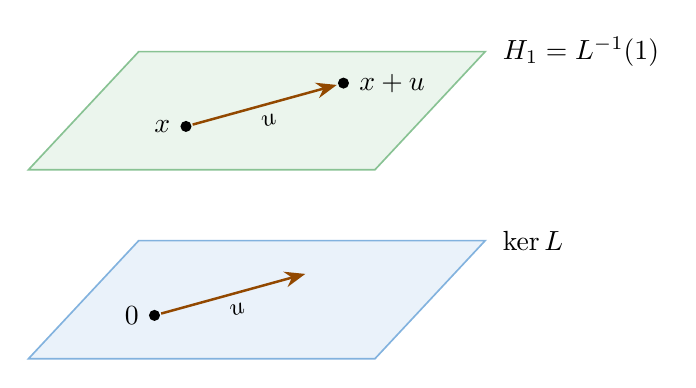
\begin{tikzpicture}
  \def\P{(0,0) -- (4.4,0) -- (5.8,1.5) -- (1.4,1.5) -- cycle}
  \fill[cB!10] \P; \draw[cB!60,line width=0.6pt] \P;
  \begin{scope}[yshift=2.4cm]
    \fill[cC!10] \P; \draw[cC!60,line width=0.6pt] \P;
  \end{scope}
  \coordinate (o) at (1.6,0.55); \coordinate (u) at (2.0,0.55);
  \coordinate (x) at (2.0,2.95);
  \draw[disp,cA] (o) -- node[lab,below]{$u$} ($(o)+(u)$);
  \draw[disp,cA] (x) -- node[lab,below]{$u$} ($(x)+(u)$);
  \node[pt,label=left:$0$] at (o) {};
  \node[pt,label=left:$x$] at (x) {}; \node[pt,label=right:$x+u$] at ($(x)+(u)$) {};
  \node[anchor=west] at (5.9,1.5) {$\ker L$};
  \node[anchor=west] at (5.9,3.9) {$H_1=L^{-1}(1)$};
\end{tikzpicture}
\end{document}
